\fancyhead{}
\fancyfoot{}
\cfoot{\thepage}


\lhead{Método}
% \chapter{Método}
\chapter{Predicción de la  demanda}
En esta sección, se describirán los métodos utilizados para llevar a cabo la investigación sobre la predicción de compras a parir de un historial de ventas.

\section{Preprocesamiento de datos}

Los datos usados para generar el modelo fueron proporcionados por la empresa gastronomica “Poroto”. La misma proporcionó el dataset para ser usado con fines académicos, los datos presentan las ventas diarias para los diferentes productos  cuenta con 6 meses de registro desde el 17 de abril del 2023 hasta el 15 de octubre del 2023.

Los datos originales suministrados están conformados por los siguientes datasets: 
\begin{itemize}
  \item productos.csv 
  \item ventas.csv
\end{itemize}

Los datos vienen organizados en forma tabular, cada archivo presenta información separada relacionada con los diferentes productos y el registro de ventas histórico.

\vspace{1\baselineskip}
\textbf{productos.csv}

Estructura inicial de la tabla de productos (informacion de los 5 primeros productos(Fig. \ref{fig:priemeros_5productos})).

\begin{figure}[H]
  \begin{center}
    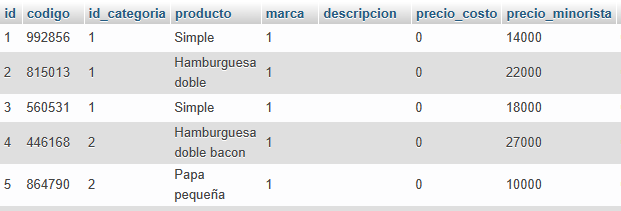
\includegraphics[scale=0.90]{./tabla_producto.png}
    \caption{Estructura inicial de la tabla productos.csv}
    \label{fig:priemeros_5productos}
  \end{center}
\end{figure}

\textbf{ventas.csv}

Estructura inicial de la tabla de ventas(con información de 6 registros (Fig. \ref{fig:ventas_original})).

\begin{figure}[H]
  \begin{center}
    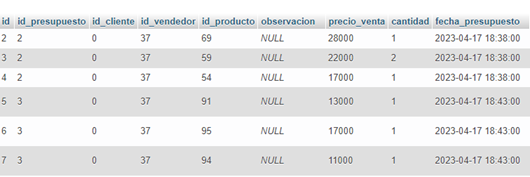
\includegraphics[scale=0.90]{./tabla_inicial_venta.png}
    \caption{Estructura inicial de la tabla  ventas.csv}
    \label{fig:ventas_original}
  \end{center}
\end{figure}

% \section{Enfoque}
% El desarrollo de un sistema de compras inteligentes que utiliza un histórico de ventas como fuente principal de información. El objetivo principal es optimizar la gestión de insumos gastronómicos.

% \begin{itemize}
% \item Recopilación y análisis de datos cuantitativos de ventas históricas para desarrollar un modelo predictivo. Esto abarcaría la identificación de patrones de ventas, el uso de algoritmos de aprendizaje automático para predecir futuras compras y la evaluación de la precisión del sistema. 
% \item Aplicación de métricas cuantitativas para evaluar el rendimiento del sistema en términos de eficiencia, impacto en las ventas y beneficios para la entidad objeto de estudio.

% \end{itemize}

% \section{Alcance de la investigación cuantitativa}
% El alcance de esta investigación descriptiva se enfoca en proporcionar una visión detallada y exhaustiva de la aplicación de un sistema inteligente de gestión de compras basado en el histórico de ventas en un local gastronómico ubicado en Ciudad del Este. 
% Se describirá el proceso de recopilación de datos históricos de ventas, incluyendo la fuente de los datos, el periodo de tiempo cubierto y la naturaleza de la información registrada.
% Se proporcionará una descripción completa de cómo opera el sistema inteligente computarizado, incluyendo su arquitectura, algoritmos de pronóstico, y la forma en que utiliza los datos históricos para generar predicciones de demanda.


\section{Análisis de los datos }
\section{Definición de variables de entrada y salida}
\section{Lectura y escalado del dataset en Python}
\section{Distribución del conjunto de datos}
\section{Aplicación y comparación de técnicas ML}
\subsection{Regresión lineal}
\subsection{LSTM}
\section{Afinación de hiperparámetros con base en porcentaje de pérdida RMS}


Cuenta con 3.840 registros de ventas que agrupados por fecha dan un total de 185 registros, que corresponden a la cantidad de ventas diarias del prodcuto mensionado organizados por fechas desde el 17 de abril de 2023 hasta el 15 de octubre de 2023.

Proporciona información de 5  productos, el dataset contiene 2 columnas: id, producto. El primero representa un identificador único para cada producto que posteriormente me permitirá relacionarlo con otras tablas, el segunto indica el nombre del producto.

\begin{figure}[H]
  \begin{center}
    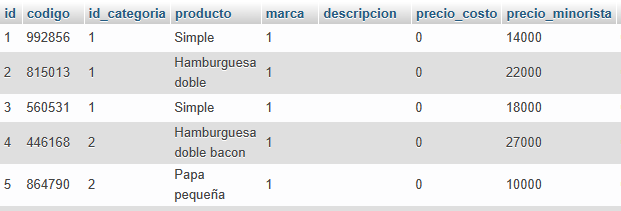
\includegraphics[scale=0.90]{./tabla_producto.png}
    \caption{productos.csv(Los primeros 5 productos)}
    \label{fig:priemeros_5productos}
  \end{center}
\end{figure}


En la tabla \ref{tab:productos} se muestra una descripción de cada una de las columnas de productos.

\begin{table}[H]

  \begin{tabular}{|c|l|}  % Usamos "l" para alinear a la izquierda
    \hline
    \rowcolor{gray!50} \textbf{Columna} & \textbf{Descripción} \\
    \hline
    id &  el id del producto (identificador unico)\\
    producto & el nombre del producto \\
    \hline
  \end{tabular}
  \centering
  \caption{ Descripción columnas productos.csv}
  \label{tab:productos} % Asigna una etiqueta a la tabla
\end{table}

  En la tabla \ref{tab:ventas} se muestra una descripción de cada una de las columnas de ventas.
  \begin{table}[H]
  \begin{tabular}{|c|l|}  % Usamos "l" para alinear a la izquierda
    \hline
    \rowcolor{gray!50} \textbf{Columna} & \textbf{Descripción} \\
    \hline
    mes &  variable mes Rango(1-12)\\
    dia & variable dias del mes Rango(1-31)\\
    dia\_semana & variable dia de la semana Rango(0-6)\\
    dia\_festivo & variable dia festivo Rango(0-1)\\
    estacion & variable estaciones del año Rango(0-3)\\
    producto & el id del producto\\
    \hline
  \end{tabular}
  \centering
  \caption{ Descripción columnas ventas.csv}
  \label{tab:ventas} % Asigna una etiqueta a la tabla
\end{table}

% \section{Analítica descriptiva}
El objetivo principal de esta etapa es explorar y comprender en profundidad los datos, lo que resulta fundamental para una sólida preparación y análisis de los mismos. Esta comprensión más profunda del problema de negocio nos permitirá seleccionar modelos de predicción y tomar decisiones más fundamentadas. Durante el proceso de limpieza y preparación de los datos, se han identificado características relevantes que proporcionarán información valiosa para las fases posteriores del análisis y la toma de decisiones.

\vspace{1\baselineskip}
Grafico en violín \ref{fig:grafico_violin} para asegurar que todas las variables de entrada estén escaladas entre 0 y 1 incluyendo el set train,validación y test.
\begin{figure}[H]
  \begin{center}
    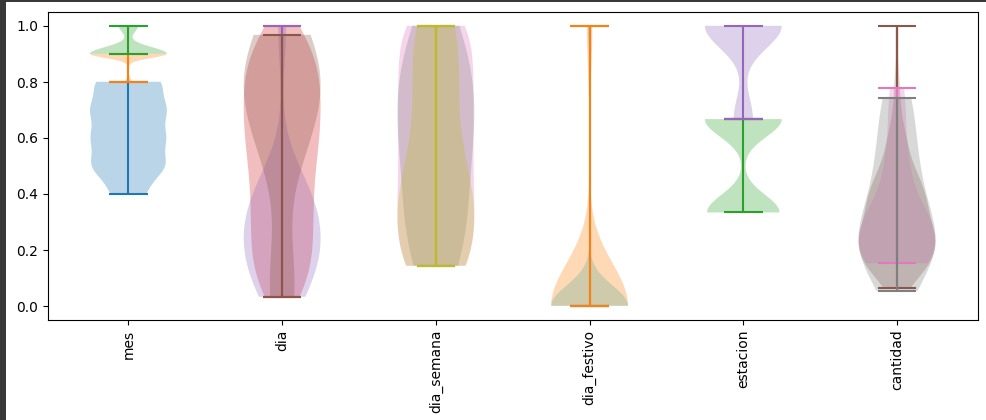
\includegraphics[scale=0.50]{./grafico_violin.jpg}
    \caption{Grafico en violín incluyendo los tres set train, validación y test}
    \label{fig:grafico_violin}
  \end{center}
\end{figure}

\vspace{1\baselineskip}
Gráfico en violín \ref{fig:grafico_violin_salida} para asegurar que los datos de salida también estén escaladas correctamente
\begin{figure}[H]
  \begin{center}
    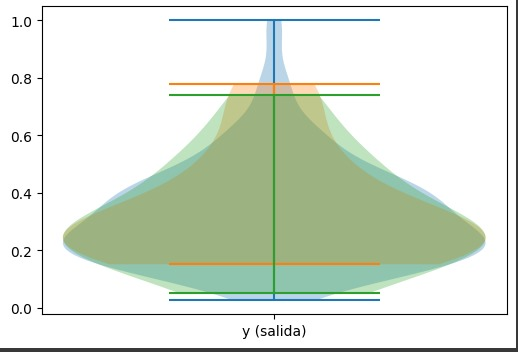
\includegraphics[scale=0.50]{./grafico_violin_salida.jpg}
    \caption{Gráfico en violín de los datos de salida escaladas}
    \label{fig:grafico_violin_salida}
  \end{center}
\end{figure}
% \section{Conjunto de datos}

% Cuenta con 3.840 registros de ventas que agrupados por fecha dan un total de 185 registros, que corresponden a la cantidad de ventas diarias del prodcuto mensionado organizados por fechas desde el 17 de abril de 2023 hasta el 15 de octubre de 2023. 

Se  empleó  un  conjunto  de  datos  recopilados  a  partir  del  número  diario  de  productos vendidos,  obtenido  de la empresa gastronomica que proveyo los datos para el analisis y predicción de la misma, es importante destacar que el conjunto de datos es continuamente actualizado, sin embargo, para los propósitos de esta investigación, se consideró un conjunto de datos con 180 registros que cubren el período desde 17 de Abril del 2023 hasta 15 de Octubre del 2023 de un producto en especifico “hamburgesa simple”.

Como el objetivo de este proyecto consiste en predecir las ventas del dia, se realiza una gráfica \ref{fig:serie_completa}, la cual nos permite ver la serie temporal de las ventas del producto mencionado. 

\begin{figure}[H]
  \begin{center}
    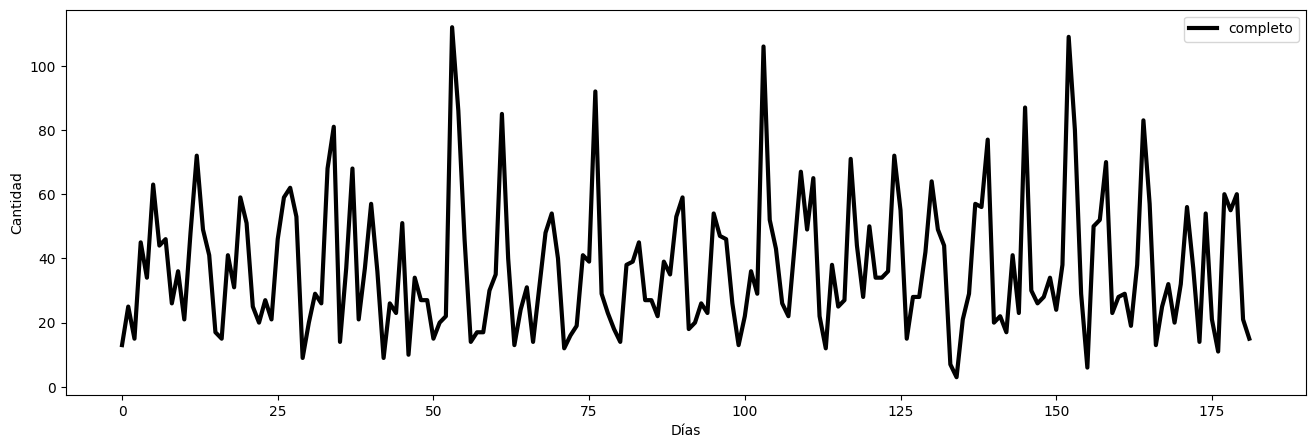
\includegraphics[scale=0.40]{./serie_normal_completa.png}
    \caption{Serie temporal de las ventas totales por día}
    \label{fig:serie_completa}
  \end{center}
\end{figure}

Posteriormente, se dividió el conjunto de datos en tres grupos: entrenamiento, validación y prueba. El grupo de entrenamiento comprendió 148 registros que cubren desde 17 de abril hasta el 9 de septiembre. El grupo de validación incluyó 18 registros, desde 10 de septiembre hasta el 29 de septiembre  y el conjunto de prueba 19 registros desde el 30 de septiembre hasta 18 de octubre.

\begin{figure}[H]
  \begin{center}
    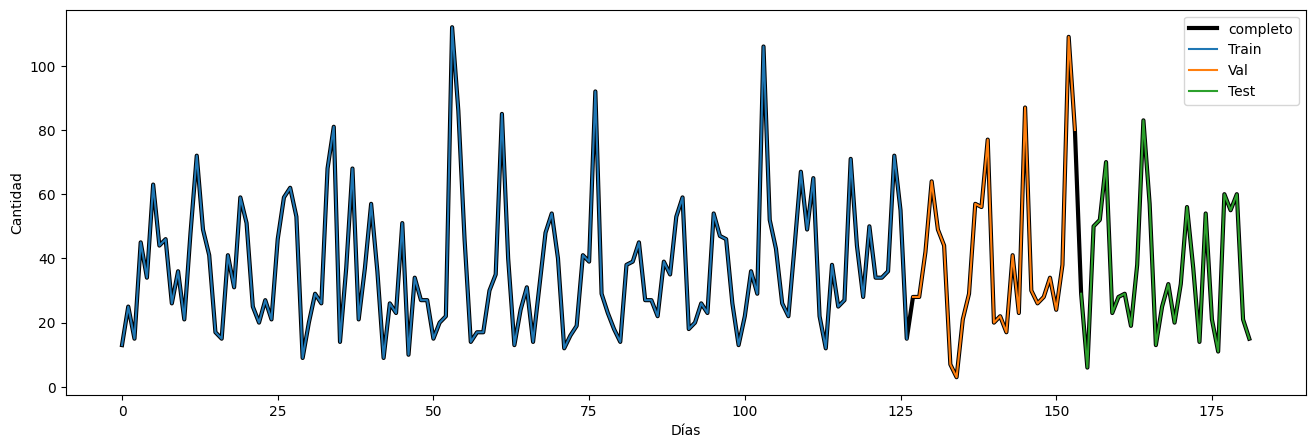
\includegraphics[scale=0.40]{./serie_normal_dividida.png}
    \caption{Distribución de los datos, ventas totales por día.}
    \label{fig:distribucion_datos}
  \end{center}
\end{figure}

\textbf{Lista de requisitos:}

\begin{itemize}
% \item Registro de usuarios(Alta, Baja, Modificaciones).
\item Registro de productos (Alta, Baja, Modificaciones).
\item Registro de insumos(materia prima) (Alta, Baja,Modificaciones). 
\item Registro de pedidos/ventas (Alta, Baja, Modificaciones).
\item Generación de Informes Personalizados: Debe permitir la creación de informes personalizados que muestren datos específicos para análisis.
\item Análisis de Tendencias: Debe ser capaz de identificar tendencias y patrones en las ventas de insumos, lo que facilita la toma de decisiones basadas en datos.

\end{itemize}
\begin{figure}[H]
    \begin{center}
      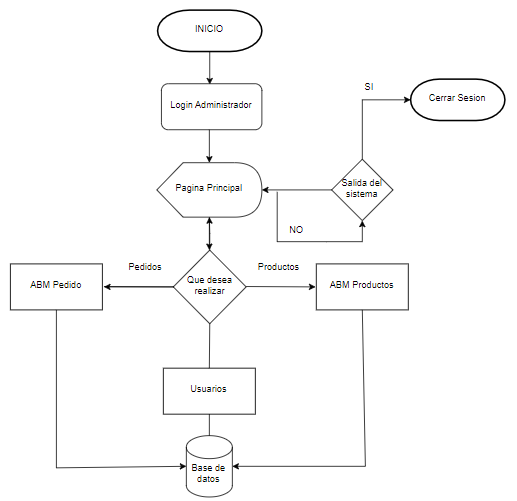
\includegraphics[scale=0.90]{./diseño_procedural.png}
      \caption{Diseño procedural.}
      \label{fig:diseño_procedural}
    \end{center}
  \end{figure}
  
% \section{Librerias de uso común en Mching Learning}
A continuación se instalara y actualizaran las principales librerias mas utilizadas cuando se realizan programas de inteligencia artificial.

\begin{itemize}
  \item \textbf{TensorFlow:} Es una plataforma de código abierto de un extremo a otro para el aprendizaje automático. Tiene un ecosistema integral y flexible de herramientas, bibliotecas y recursos comunitarios que permite a los investigadores impulsar lo último en ML y a los desarrolladores crear e implementar fácilmente aplicaciones basadas en ML.
  Es ampliamente utilizada para desarrollar y entrenar modelos de redes neuronales, incluyendo modelos LSTM (Long Short-Term Memory).
  \item \textbf{Keras:} Es una interfaz de alto nivel para TensorFlow que facilita la construcción, entrenamiento y evaluación de modelos de redes neuronales, incluyendo modelos LSTM.
\end{itemize}



La función de activación utilizada para modelar la no linealidad suele ser la Unidad Lineal Rectificada (ReLU), que puede calcularse más rápido que las funciones tangentes sigmoideas o hiperbólicas utilizadas tradicionalmente y también ofrece interesantes propiedades de convergencia.
% \subsection{Alcance exploratorio.}
% La medida de este alcance abarca la exploración de problemas generalmente poco conocidos, a veces difíciles de conocer.

% \subsection{Alcance descriptivo.}
% La medida de este alcance abarca la descripción del fenómeno, situación, contexto o evento; detalla cómo es y cómo se manifiesta. Busca especificar propiedades, características y rasgos importantes. Describe tendencias de un grupo o población. Es útil para mostrar con precisión los ángulos o dimensiones de un fenómeno, suceso, comunidad, contexto o situación.

% \subsection{Alcance correlacional.}
% La profundidad de este alcance busca establecer relaciones entre variables sin precisar sentido de causalidad, es decir, no analiza relación causal.

% Un ejemplo de este alcance es una investigación que busca averiguar cómo se relacionan las calificaciones de los alumnos de un grado, en las asignaturas: Castellano y Matemática.

% \subsection{Alcance explicativo.}
% La profundidad de este alcance busca establecer relaciones entre variables precisando sentido de causalidad, es decir, analiza relación entre causa y efecto entre variables.

% Un ejemplo de este alcance es una investigación que busca averiguar la relación entre urbanización y alfabetismo en un país, para ver qué variables macrosociales definen el grado de alfabetización de la población del país.

% \section{Diseño}
% Es el plan o estrategia que se desarrolla para obtener la información que se requiere en una investigación, generalmente para verificar la hipótesis. La precisión, amplitud y profundidad de la información obtenida varía en función del diseño elegido \cite{sampieri}.

% En la literatura sobre investigación cuantitativa es posible encontrar diferentes clasificaciones de los diseños; los autores \cite{sampieri} adoptan la siguiente clasificaciòn: investigación experimental e investigación no experimental. A su vez, la primera puede dividirse de acuerdo con las clásicas categorías de Campbell y Stanley (1966) en: preexperimentos, experimentos ``puros'' y cuasiexperimentos. La investigación no experimental, siempre de acuerdo con \cite{sampieri}, se subdivide en diseños transversales y diseños longitudinales.

\vspace{.5 cm}

% \textbf{Ejemplo de diseño en una investigación tecnológica formativa.}

% Aún más que en la investigación en ciencias básicas, es en la investigación tecnológica donde se puede apreciar la importancia del diseño para obtener un buen producto o servicio. Cabe entonces ilustrarlo con un ejemplo tomado dentro de esta última forma de investigación desde la referencia \cite{lan}.

\vspace{.5 cm}


% \textbf{\emph{Metodología para implementar red de área local. (\gls{lan}\@)}}\footnote{Por brevedad, solo se desarrolla la etapa de diseño.}




% Hoy en día, como nunca antes, el ser social necesita estar informado. Para estudiar problemas y tomas de decisiones es necesario disponer de datos precisos, en el lugar y en el instante preciso. En gran medida se logra lo anterior con las redes de computadoras, cuyo objetivo fundamental es compartir recursos e información pues ofrecen acceso a servicios universales de datos tales como: bases de datos, correo electrónico, transmisión de archivos y boletines electrónicos; eliminando el desplazamiento de los individuos en la búsqueda de información y aumentando la capacidad de almacenamiento disponible por cada usuario en un momento determinado.

% Un gran porcentaje de las redes de computadoras se usan para la transmisión de información científica siendo una vía rápida y económica de divulgar resultados y de discutir con otros especialistas afines sobre un tema en cuestión. En este trabajo en particular se aborda la metodología a seguir para la implementación de redes de computadoras de área local; las cuales cumplen todos los objetivos planteados a una escala reducida ya que son propiedad de una sola organización (un solo centro administrativo o fabril) abarcando zonas geográficas de algunos kilómetros como máximo. La experiencia en el campo de \glspl{lan} en el ámbito universitario, donde las mismas se emplean para la gestión administrativa y económica, para la transmisión de información científica y para la enseñanza; ha dejado claro que el diseño, la instalación y puesta a punto de una \gls{wan} suele ser un proceso cuidadoso del cual depende en grado sumo que se cumplan los objetivos para los que se invirtió en dicha red.

Para su comprensión el trabajo se divide en cinco partes o etapas:
\begin{itemize}
\item Etapa de estudio,
\item Etapa de diseño.\footnote{Solo se desarrolla esta etapa.}
\item Etapa de elaboración de la solicitud de oferta y selección del vendedor,
\item Etapa de instalación y puesta en funcionamiento,
\item Etapa de análisis de las prestaciones y evaluación de los resultados.
\end{itemize}
 
% Una vez concluida la primera etapa y aprobado el presupuesto de la red es necesario realizar la etapa del \textit{diseño} de la \gls{lan} para lo cual se deben seguir los siguientes pasos:

\renewcommand{\labelitemi}{$-$}

% \begin{itemize}
% \item Seleccionar la(s) topología(s) y norma(s) de red a emplear,
% \item Seleccionar el soporte de transmisión a utilizar,
% \item Analizar la necesidad de emplear técnicas de conectividad,
% \item Considerar ampliaciones futuras de la red,
% \item Realizar una evaluación primaria del tráfico,
% \item Contemplar las necesidades del personal involucrado en la red,
% \item Modificar, de ser necesario, el flujo de la información y seleccionar el software de aplicación.
% \end{itemize}

% \textit{Seleccionar la topología.} Este paso, el cual es dependiente de los resultados del anterior. Las tres topologías más empleadas son: bus, estrella y anillo; mientras que las normas más comunes son: Ethernet, Token Ring y ArcNet. La selección de los aspectos anteriores trae aparejado escoger la velocidad de transmisión, la distancia máxima a emplear, el método de control de acceso al medio, etc. La elección se realiza a partir de la necesidad particular y de un amplio conocimiento de las topologías y normas existentes. 

% \textit{Seleccionar el Soporte de Transmisión.} Esto está muy relacionado con la norma a emplear y con las características de los puntos a conectar. Es vital realizar una selección adecuada pues una opción equivocada comprometería la eficacia y la velocidad de la transferencia de datos. Para la elección de uno u otro medio de transmisión se debe tomar entre otras cosas las dimensiones de la instalación, el costo, la evolución tecnológica estimada, la facilidad de instalación y el grado de hostilidad electromagnética presente en el entorno. 

% Aunque el \gls{sored}  (del inglés NOS: Netware Operating System) NetWare predomina en el mundo, éste no es siempre la elección adecuada, debido a sus costos y características. En el mercado existen otros \glspl{sored} tales como: LAN Manager, LANServer, LANtastic, Vines, LINUX, Windows NT Server, Windows 2000 Server, etc.; los cuales poseen una determinada cuota de mercado. Para seleccionar el SOR adecuado se debe tener en cuenta:

% \begin{itemize}
% \item El nivel de confidencialidad que brinda a los datos,
% \item Si es del tipo cliente-servidor o de igual a igual,
% \item Grado de tolerancia a fallos que posee,
% \item Memoria RAM necesaria en el servidor y en las estaciones de trabajo,
% \item Facilidades de administración y diagnóstico que brinda,
% \item Si posee o no sistema de correo electrónico,
% \item Características de manipulación de colas de impresión.
% \end{itemize}

% \textit{Analizar la necesidad de emplear técnicas de conectividad.} Esto estará en función de las dimensiones de la organización, del tráfico a cursar y el tipo de equipamiento a interconectar entre otros aspectos. Es necesario conocer en profundidad dichas técnicas para realizar una adecuada selección entre repetidores, puentes, ruteadores, compuertas, servidores de acceso, etc. y lograr su correcta ubicación. La mejor solución muchas veces hace uso de más de un tipo de dispositivo de interconexión.

% \textit{Considerar ampliaciones futuras de la red.} Aún cuando de forma inmediata no sea necesario extender la red ni conectarse a otros, ésta debe poseer la base para que a partir de ella, y en cualquier momento sea posible una ampliación o llegar a formar parte de otras redes.

% \textit{Realizar una evaluación primaria del tráfico.} Aquí debe estimarse el tráfico que circulará en la red y analizar si el mismo no afecta el tiempo de acceso a la información ya otros recursos compartidos. Es importante que una vez instalada y puesta en funcionamiento la \gls{lan} se efectúen periódicamente estudios de este tipo.

% \textit{Contemplar las necesidades del personal involucrado en la red.} Esto es muy importante pues en última instancia éste será el personal que utilizará la red y por lo tanto deben quedar satisfechas sus necesidades de forma tal que la nueva red sea un elemento que facilite su trabajo.

% \textit{Modificar de ser necesario el flujo de información y seleccionar el software de aplicación.} Esto implica la modificación, como última opción, de la manera en que la información circula dentro de la organización y la definición del software de aplicación necesario, ya sea comercial o aquél que se encargará al personal especializado; que conozca las particularidades de la programación en ambiente multiusuario. El software encargado o adquirido debe ser de fácil instalación y aprendizaje. Además se debe velar porque sea posible tener acceso a posteriores actualizaciones y que éstas no sean caras.

% \section{Lenguajes de programación}

% \subsection{Python}
% Python es un lenguaje de programación potente y elegante
% que sea fácil de leer y de entender\cite{python2021python}.

% Tiene estructuras de datos de alto nivel eficientes y un simple pero efectivo sistema de programación orientado a objetos. La elegante sintaxis de Python y su tipado dinámico, junto a su naturaleza interpretada lo convierten en un lenguaje ideal para scripting y desarrollo rápido de aplicaciones en muchas áreas, para la mayoría de plataformas.

% Python se destaca en el ámbito de la inteligencia artificial debido a su capacidad para gestionar conjuntos de datos voluminosos y su facilidad de programación. Su sintaxis concisa y legible lo convierte en una elección ideal para crear prototipos de forma rápida, dinámica y comprensible.
% Además de su amplia popularidad, la razón principal para adentrarse en Python en el contexto del aprendizaje automático es, indiscutiblemente, su vasto ecosistema de recursos previamente desarrollados. 

% \paragraph{Pandas:}
% Es una biblioteca de código abierto que proporciona estructuras de datos flexibles y herramientas de análisis de datos para Python. Su principal estructura de datos es el DataFrame, que permite organizar datos en tablas bidimensionales. Pandas es ampliamente utilizado para la limpieza, manipulación y análisis de datos tabulares, lo que lo hace esencial en el análisis de datos.

% \paragraph{NumPy:}
% Es una biblioteca fundamental para el cálculo numérico en Python. Proporciona soporte para arreglos multidimensionales (llamados ndarrays) y una amplia gama de funciones matemáticas para operaciones en estos arreglos. NumPy es crucial para realizar cálculos numéricos eficientes y es la base de muchas otras bibliotecas de análisis de datos en Python.

% \paragraph{Matplotlib:}
% Es una biblioteca de visualización que permite crear gráficos estáticos de alta calidad. Proporciona una variedad de tipos de gráficos, desde gráficos de líneas y barras hasta histogramas y gráficos de dispersión. Matplotlib es ampliamente utilizado para visualizar datos y resultados en el análisis de datos.

% \paragraph{Seaborn:}
% Es una biblioteca de visualización basada en Matplotlib que simplifica la creación de gráficos estadísticos atractivos. Ofrece una interfaz de alto nivel para crear fácilmente visualizaciones complejas y atractivas, lo que la hace útil para el análisis exploratorio de datos y la presentación de resultados.

% \paragraph{Scikit-learn:}
% Es una biblioteca de aprendizaje automático que proporciona herramientas para tareas comunes de aprendizaje automático, como clasificación, regresión, clustering y selección de modelos. También incluye utilidades para la evaluación de modelos y el preprocesamiento de datos, lo que la convierte en una biblioteca esencial para el análisis de datos relacionados con el aprendizaje automático.

% \paragraph{StatsModels:}
% Es una biblioteca que se utiliza para realizar análisis estadísticos y modelado en Python. Está especialmente orientada a tareas como la regresión lineal y logística, análisis de series temporales y pruebas estadísticas. Es útil para realizar análisis estadísticos rigurosos en el contexto del análisis de datos.

% \paragraph{SciPy:}
% Es una extensión de NumPy que proporciona funcionalidades adicionales para cálculos científicos y técnicos. Incluye módulos para optimización, interpolación, integración numérica, álgebra lineal, transformadas y más. Es una biblioteca esencial para aplicaciones científicas y de ingeniería que involucran cálculos numéricos.

% \paragraph{Plotly:}
% Es una biblioteca que permite crear gráficos interactivos y visualizaciones web en Python. Es útil para crear visualizaciones interactivas para el análisis exploratorio de datos y la presentación de resultados en aplicaciones web.

% \paragraph{Bokeh:}
% Es otra biblioteca para crear gráficos interactivos y aplicaciones web basadas en datos. Ofrece una amplia gama de herramientas para crear visualizaciones interactivas y es especialmente útil para proyectos que requieren interfaces de usuario interactivas.

% \paragraph{Dask:}
% Es una biblioteca que se utiliza para el procesamiento paralelo y distribuido de datos en Python. Permite trabajar con conjuntos de datos grandes y realizar operaciones complejas de manera eficiente en clústeres de computadoras.

% \paragraph{TensorFlow y PyTorch:}
% Si bien estas bibliotecas son conocidas principalmente por el aprendizaje profundo, también se utilizan en tareas de procesamiento y análisis de datos cuando se trabajan con modelos de redes neuronales. Proporcionan herramientas para construir, entrenar y evaluar modelos de aprendizaje automático y profundo.

% Estas bibliotecas forman la base del ecosistema de análisis de datos en Python y son esenciales para una variedad de tareas en ciencia de datos, análisis de datos y aprendizaje automático.

% \subsection{PHP}
% Es un lenguaje de programación ampliamente utilizado en el desarrollo web. Se destaca por su capacidad para crear aplicaciones web dinámicas e interactivas\cite{cobo2005php}.

% Ofrece diversas ventajas que lo hacen atractivo en el desarrollo web:

% \paragraph{Facilidad de aprendizaje:}
% Tiene una sintaxis simple y legible, lo que facilita su aprendizaje, especialmente para principiantes en programación.
% \paragraph{Amplia comunidad y soporte:}
% Cuenta con una gran comunidad de desarrolladores y abundantes recursos en línea, incluyendo bibliotecas y frameworks, lo que agiliza el desarrollo.
% \paragraph{Interacción con bases de datos:}
% Brinda soporte integrado para la mayoría de las bases de datos populares, lo que lo hace ideal para aplicaciones que gestionan datos.
% \paragraph{Versatilidad:}
% Se integra fácilmente con HTML y otros lenguajes web, permitiendo una amplia gama de aplicaciones y funcionalidades.
% \paragraph{Plataforma cruzada:}
% Es compatible con varias plataformas y sistemas operativos, lo que lo hace altamente portátil.
